\section{Preliminary Validation}
\label{sec:preliminary-validation}

While the complete execution of the 30 experimental iterations and their subsequent statistical analysis are reserved for future work, the PANOPTES testbed has been successfully instantiated and validated. Preliminary executions confirm that the infrastructure components interact as mathematically specified in the architectural design.

\begin{figure}[htbp]
  \centering
  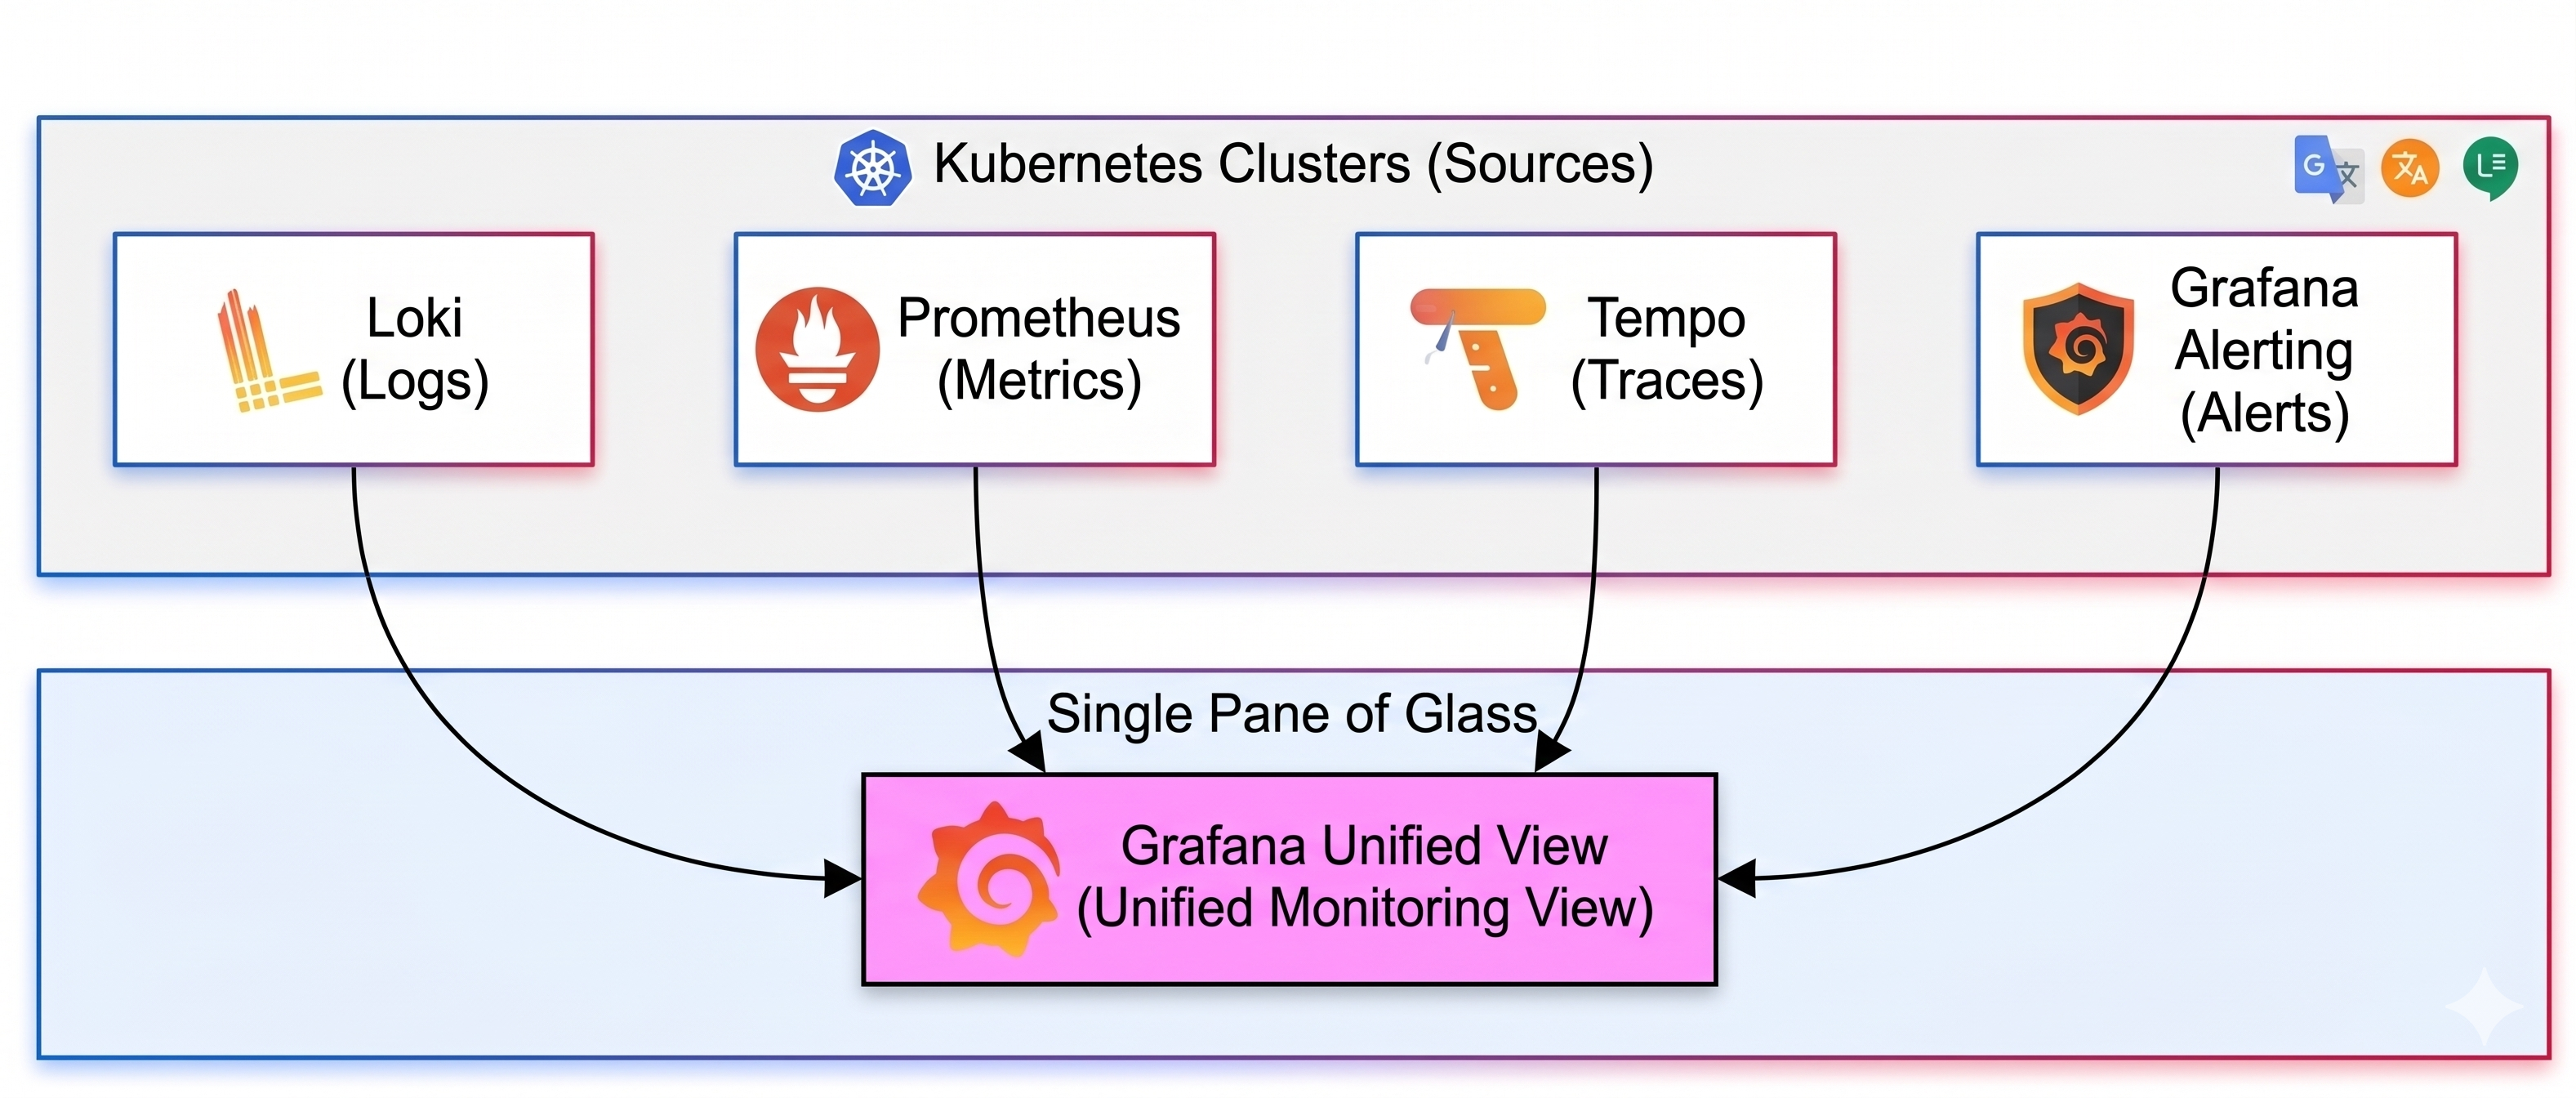
\includegraphics[width=0.9\textwidth]{images/experiment/grafana_preliminary.png}
  \caption{Single Pane of Glass of Grafana}
  \label{fig:grafana_preliminary}
\end{figure}

Figure \ref{fig:grafana_preliminary} demonstrates the ``Single Pane of Glass'' operational state, proving that the OpenTelemetry collectors are actively scraping the target microservices and successfully forwarding the telemetry data to the Prometheus, Loki, and Tempo backends. Furthermore, the Chaos Mesh operator has been tested and confirmed to successfully disrupt the network namespaces of the target pods without crashing the underlying K3s control plane, validating the safety of the fault injection mechanism.

The Single Pane of Glass requirement is met by Grafana. However, simply displaying independent dashboards for metrics, logs, and traces does not constitute true observability. The PANOPTES instantiation implements strict semantic correlation between these signals to directly reduce the Mean Time to Detect (MTTD).

This crucial correlation is implemented concretely through specific datasource configurations within Grafana:
\begin{itemize}
    \item \textbf{Metrics to Traces via Exemplars:} The Prometheus datasource is configured to extract \texttt{traceID} values from metric exemplars. When an SRE identifies a latency spike in a metric panel, they can click the exemplar data point. This action automatically queries the Tempo datasource using that exact \texttt{traceID}, instantly rendering the distributed trace without requiring the user to manually copy and search IDs across different tools.
    \item \textbf{Traces to Logs:} The Tempo datasource is configured with a \textit{Trace to Logs} mapping. From a specific span within a failing trace, Grafana automatically generates a LogQL query for Loki. It filters the logs by the identical \texttt{traceID} and Kubernetes namespace, bridging the cognitive gap between "knowing a request failed" and "seeing the exact stack trace or error log that caused it".
\end{itemize}

These integrated dashboards are provisioned dynamically as code via Helm, ensuring the correlation logic is reproducible across any cluster deploying the PANOPTES architecture.